\chapter{Learning speech acts}
\label{chap:eng-sp}
As we have discussed in the last two chapters, pragmatics is crucial for children to learn clause type categories, and that even with 80\% of noise in the speech act data, learners could still benefit from this source of information. This chapter investigates non-clause type cues in the input that might be helpful for children to identify different speech acts, in particular questions. Are there any non-clause type cues? How informative are these non-clause type cues? If children use these cues, is it possible for them to predict 20\% of the data? I focus on three types of cues, prosody, speech gap, and eye gaze. 

This chapter is organized as follows: Section~\ref{sec:engsp:background} reviews the three cues in detail, what kind of pattern might be correlated with different speech acts, and previous evidence for children's perception of these cues. I report results from a corpus study with Providence Corpus (\cite{ProvidenceCorpus}), which I used in Chapter~\ref{chap:eng-cl}. % I find that...
Section~\ref{sec:engsp:discussion} concludes the chapter.


\section{Background}
\label{sec:engsp:background}
\subsection{Prosody}
\label{sec:engsp:bg:prosody}

Previous studies show that children are sensitive to prosodic distinctions since birth. %Since birth, babies have been shown to be particularly sensitive to pitch and other prosodic differences in speech. Research highlights that infants are able to use prosodic cues consistently some months after birth, not only in terms of sensitiveness to prosodic acoustic features (Bosch & Sebastián-Galles, 2001; Fernald & Kuhl, 1987; Jusczyk et al., 1993; Mehler et al., 1988; Nazzi et al., 1998; Ramus et al., 2000) b


From as early as 6 months old, infants are found to be able to use these distinctions to distinguish different speech acts since birth. From the comprehension side, infants are found to be able to use prosodic cues to distinguish clause types and speech acts. \textcite{frota2014} show that as young as 6 months old, infants are sensitive to the prosodic distinction between polar interrogatives and declaratives, which is the only cue that distinguishes these two clause types. \textcite{geffenmintz2011} find that when given a combination of word order and prosodic cues, English-acquiring 7-month-olds can distinguish polar interrogatives from declarative assertions. \textcite{soderstrom2005clause} test English-speaking infants between 4.5 months and 2 years old (average 14 months old), and find that they are sensitive to the distinction between declaratives with a falling a rising contour. \textcite{} show that 14 month-olds English-acquiring respond differently to a rising contour, and only learn novel labels to objects if the word is pronounced with a rising contour.\footnote{Their studies uses stimuli created with Mandarin lexical contours, in particular the rising tone (tone 2) and the falling tone (tone 4). Although the rising tone is very similar to English polar-interrogative rise, and the falling tone similar to English declarative fall, and that 14-month-olds show different behaviors toward these two tones, it is unclear whether we can draw any conclusions about their sensitivity to English polar interrogative rise.}


On the production side, studies have found that children are able to use different prosodic contours for different functions from when they start speaking. \textcite{menyuk1969prosody} analyze the prosodic contours of one child's utterances, and annotates their perceived speech acts between 18  and 20 months, and find that even though the utterances are mostly one word or two words, there's a correlation between the intended speech act and prosody. For example, an intended request with a one-word utterance ``door!" is typically associated with a sharp rise and then fall; the same utterance as a question tends to end with a rising intonation. Since the speech act labels in the study are annotations by adults inferred from one-word utterances, it is unclear whether these are actually the speech acts that the child perform, and the conclusion seems to be that adults systematically associate certain prosodic contours to \aqrs{}, even with one-word utterance. Nonetheless, it seems that at the child is using different prosodic contours at this age, and it is possible that these contours are systematically associated with different speech acts. 
% Esteve-Gibert & Prieto (2013) analysed a total of 2,701 vocalizations from a longitudinal corpus of four Catalan-babbling infants aged 0;7 to 0;11. The results also showed that infants use different prosodic patterns to distinguish communicative from investigative vocalizations and to express intentionality. Specifically, they found that requests and expressions of discontent displayed wider pitch range and longer duration patterns than responses or statements. 

%Studies on the prosody-pragmatics interface show that children around the two-word stage display an emerging complex inventory of intonation contours with an adult-like intentional meaning (Chen & Fikkert, 2007; Frota, Vigario, & Cruz, to appear; Prieto et al., 2012).  

Furthermore, children seem to associate the rising contour with response elicitation. \textcite{flax1991prosody} conduct a longitudinal study observing three children interacting with their mothers before they can speak, when they have a vocabulary of 10 words, and when their vocabulary consists of 50 words, and code whether the child's utterance (or vocalization, at the pre-verbal stage) is produced with a final rise. They find when children request a response from their addressee, they tend to produce the utterance with final rise. 

Previous studies have also shown that there are prosodic cues that distinguish clause types and speech acts, in particular, between polar interrogatives and declaratives, in child-directed speech. \textcite{geffenmintz2017final} show that, polar interrogatives and declaratives differ in the pitch of the last two syllables, with polar interrogatives generally have a rising contour; they also find that there is no distinction between \twh-interrogatives and declaratives in the last two syllables. \textcite{chianggeffenmintz2018initial} examines sentence-initial prosodic cues, and find that polar interrogatives and declaratives both have a higher starting pitch than declaratives, and that echo \twh-questions tend to have a higher pitch than other types of questions. %These studies only looked at the duration, F0, and intensity of the last two and the first syllables; there might be 

In summary, prosodic might help children distinguish different speech acts, and that children can perceive these cues. In particular, there might be cues at sentence-final and sentence-initial position. We will examine the role of prosody more closely in Section~\ref{sec:engsp:corpus}, and go beyond the last two and the first syllables.

\subsection{Speech gap}
\label{sec:engsp:bg:pause}
Questions are turn-transition points (\cite{duncan1972turn} among others), and this means that speakers anticipate a change of turn after questions. In adult-to-adult conversations, this property translates to shorter speech gaps after questions in general (\cite{stivers2010,enfield2010,hilbrink2013turn} among many others). 



As early as 3 months old, infants show sensitivity to the structure of conversation. The overlap between infant vocalization and parents' speech decreases overtime, and the average gap between parent utterance and infant vocalization decreases, suggesting that they respect the turn-taking rules (\cite{hilbrink2013turn3mo}). When they start producing one-word utterances, slow down at trying to change turn, but quickly pick up the speed again as their linguistic ability develops (\cite{hilbrink2013turn}). 

%Bloom et al: four children, 21 to 36 months of age. Adjacent speech is more than anything from the beginning, Contingent speech increase over time (adjacent (immediately preceded by an adult utterance), or as nonadjacent (not immediately preceded by an adult utterance). Adjacent utterances were either contingent (shared the same topic and added new information relative to the topic of the prior utterance), imitative (shared the same topic but did not add new information), or noncontingent (did not share the same topic). Linguistically contingent speech (speech that expanded the verb relation of the prior adult utterance with added or replaced constituents within a clause)  occurred more often after questions than nonquestions. 

Studies also show that children interpret pauses as meaningful.
%Craig, Gallagher (1983): six children, 22-36mo; whether they abandon their requrest (I want a cookie) or not after the parent's initial response (neutral: you want what? Neg: no. Pause) . A subset of them (older kids) abandon requrests after adult pauses for more than 1s. They conclude that this suggests that some children treat long pauses as a distinct class of speech act.

Previous studies show that parents seem to treat any vocalizations (e.g. crying, babbling) as a turn. 
%Jaffe et al. 2007:  Parents treat their infants as capable of making meaningful contributions: they take every look, vocalization, arm flail, and burp as ‘‘utterances” in the joint discourse 

%\textcite{reimchen2017} observe that parents to 14-month-olds tend to follow questions with another question. They separated utterances with 0.75s pause in-between. Infants are considered "responding" if they vocalize within 2s of parents' utterance, and 14-month-olds responded to 18% of parents' questions, and 18% of parents' assertions
%Bornstein etal.2008: parents use questions to respond to infants' vocalization starting 14-21month (mom are expecting more responses from infants)

While these studies show that parents respect turn-taking rules when interacting with pre-verbal infants, but so far little is known whether parents' speech gaps are informative of the speech act performed. Section~\ref{sec:engsp:corpus:pause} examines the correlation between the speech act of an utterance and the length of pauses after an utterance, to see if the gap between utterances is informative of an utterance's speech acts. 

\subsection{Gaze pattern}
\label{sec:engsp:bg:gaze}
%Argyle 1972: speakers use gaze for turn allocation
% gaze func- tions in dyadic encounters, such as to initiate interaction, signal address, receive addressee feedback, and coordinate turn transi- tions  Kendon, 1967, 1990; Argyle et al., 1973; Cary, 1978; Duncan et al., 1979; Goodwin, 1980; Bavelas et al., 2002; Lerner, 2003; Rossano et al., 2009) 

While these studies show that infants can perceive parents' direction of eye gaze, and that adults use eye gaze for turn allocation, but so far little is known whether parents' gaze pattern correlates with turn allocation, and furthermore, with the speech act of an utterance. If questions signals a transition of turn, parents' gaze should fall on the addressee--the child--more after questions. Section~\ref{sec:engsp:corpus:pause} examines parents gaze pattern during parent-child interactions, to see if this cue is informative of an utterance's speech acts.

\subsection{Interim Summary}
\label{sec:engsp:bg:summary}

\section{Corpus study}
\label{sec:engsp:corpus}


we want to examine the available signals in child-directed speech that correlate with parents' use of different speech acts. In particular

\subsection{Methods}
\label{sec:engsp:corpus:method}

\label{sec:engsp:corpus:uttgoals}
\subsubsection{Audio data}
\label{sec:engsp:corpus:audio}
\subsubsection{Video data}
\label{sec:engsp:corpus:video}


\subsection{Predictions}
\label{sec:engsp:predictions}

\subsection{Results}
\label{sec:engsp:results}



\subsubsection{Prosody}
\label{sec:engsp:results:prosody}

\subsubsection{Speech gap}
\label{sec:engsp:results:pause}

The other property of interest is that they expect responses. For conversations with pre-linguistic infants, this may mean that parents wait longer after questions for a response. Thus, in this project, we plan to measure the length of pause between parents’ consecutive utterances like (\ref{code-prag:pause}). To do so, we will first extract the consecutive turn sequences in parents’ speech. Following \cite{reimchen2017}, we define such sequences as a sequence of utterances spoken by the same speaker on the same topic. Within the sequences, we will measure the length of pauses between utterances, and see if parents pause longer after questions than after assertions. Moreover, we will code whether a question in the sequence is followed by another question, since \cite{reimchen2017} observe that parents to 14-month-olds tend to follow questions with another question. Our preliminary results show that parents are equally likely to ask another question as they are to answer their own questions, but parents tend to pause longer after questions (mean $= 1861ms$, Fig.~\ref{fg:pauses}) than assertions (mean $= 1216ms; t(347) = 2.08, p <0.05$): parents wait for responses after asking a question but proceed with the conversation after an assertion. 




\bex{code-prag:pause}
%\bxl{}
\tbf{Consecutive turn sequence}\\ 
%Alex's mother: Who’s that? [pause: 1.086s] Is that the postman?	\hfill		
\bxl
\ex You can’t take your rake on the swing but you can [pause: 0.014s] You wanna take your big bird rake on the swing? 			\hfill \tsc{Assertion -Question}
\ex You don't wanna swing? [pause: 0.23s]	You don’t have to.	\hfill \tsc{Question-Assertion}
\ex Here you use this one. [pause: 0.033s] This one works better.	\hfill \tsc{Assertion-Assertion}
\exl
\eex


%\vspace{-3ex}
%\noindent 
%\begin{figure}[H]
%\begin{center}
%	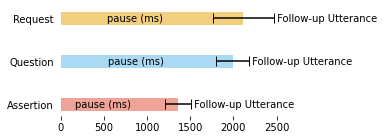
\includegraphics[width = 0.5\textwidth]{q-followup.png}
%	\caption{Duration of pause (ms) after each speech act}\label{fg:pauses}
%\end{center}
%\end{figure}

\subsubsection{Gaze pattern}
\label{sec:engsp:results:gaze}



Another consequence of the response-expectation property of questions is that by the end of a question, the speaker tends to appoint the next speaker. A common device for turn allocation is eye gaze (\citealt{argyle1972gaze, kendon1967gaze,duncan1979gaze, rossano2009gaze}), so the \hypos{} predicts that parents would engage in longer eye contact after questions than other types of speech acts. To test this, we plan to annotate, on a second-by-second basis, parents' attentional behaviors toward the child using ELAN. The annotation will be done without reference to the transcript so that the annotator is not biased by the linguistic information of the scene. For each video, the annotators will first identify the segments of the video where the parent and the child are both visible on screen, and the parent’s focus of attention is identifiable via her visual focus or head/body orientation. Then for these segments, we will annotate whether the parent is attending to the child.  


\begin{figure}[H]
\label{fg:attention}
\begin{center}
	%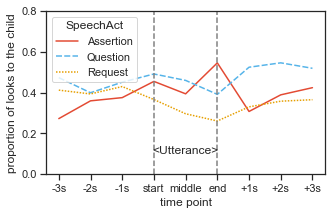
\includegraphics[width =0.4\textwidth]{q-attention.png}
	\caption{Proportion of parents' looks to the child (preliminary results)}
\end{center}
\end{figure}


Fig.~\ref{fg:attention} shows the proportion of looks to the child before and after uttering a sentence in our pilot sample: when the utterance is a question, the proportion of looks to the child is higher ($0.47$) than when it is an assertion ($0.39; t(16) = 2.53, p <0.05$) or a request ($0.35; t(16)= 4.55, p<0.001$); in the post-utterance region, the proportion of looks to the child is higher when the utterance is a question ($0.53$) than when it is an assertion ($0.37; t(4) = 4.4, p<0.05$) or a request ($0.35; t(4) = 13.2, p<0.001$). These results suggest that the predictions of the \hypos{} are borne out: parents look at the child longer after questions. Thus, despite parents asking questions whose answers they know, the characteristic turn-changing properties of questions are observable in speech pauses and speaker attention. 


\subsubsection{Informativeness of the cues}
\label{sec:engsp:results:stats}

\section{Discussion}
\label{sec:engsp:discussion}

